% Start preamble
\documentclass[12pt,a4paper]{article}
\usepackage{geometry}
 \geometry{
 a4paper,
 total={170mm,257mm},
 left=20mm,
 top=20mm,
 }
\usepackage[utf8]{inputenc}
\usepackage[T1]{fontenc}
\usepackage[pdftex]{graphicx}
\graphicspath{{./}}
\usepackage{enumitem}
\usepackage{pdfpages}
\usepackage{hyperref}
\usepackage{tikz}
\usetikzlibrary{arrows.meta, positioning, shapes.geometric,decorations.pathmorphing, calc}
\usepackage{attachfile}
\usepackage{epstopdf}
\usepackage{array}
\usepackage{multirow}
\usepackage{multicol}
\usepackage{float}
%\usepackage[table]{xcolor,colorbl}
\setlength{\textwidth}{17cm}
\setlength{\oddsidemargin}{-0.5cm}
\setlength{\evensidemargin}{-0.5cm}
%\setlenght{\headsep}{0cm}
\setlength\parindent{0pt}
%\setlength{\extrarowheight}{3pt}
\usepackage{listings}
%\usepackage{xcolor}

\input{arduinoLanguage.tex}
%%%%%% Counting oppgaves %%%%%%
 \newcount\questnum \questnum=0
 \def\oppgave{
            \advance\questnum by 1
	    \ifthenelse{\questnum>0\AND \questnum<9}
	    {
                \vskip 1cm
		\textbf{Oppgave}\hskip 5pt\the\questnum \hfill \hfill(6p)
		\vskip 3pt
		\hrule
	\vskip 0.5cm}
	{
                \vskip 1cm
		\textbf{Oppgave}\hskip 5pt \the\questnum \hfill \hfill(12p)
		\vskip 3pt \hrule \vskip 0.5cm }

		}

\begin{document}
\title{Prøve Hydraulikk \\ 2INTA Gand VGS}
\author{Faglærer: Fred-Olav Mosdal 90507684\\}
\maketitle
|
\newpage
\oppgave{}%1
\vskip 5pt 
I hydrauliske anlegg har vi energitap, hvilken energiform går dette tapet over til?
                \vskip 1cm
		\textbf{Svar}\hfill
		\vskip 3pt
		\hrule
		\vskip 10pt
I hydrauliske anlegg går energitapet primært over til \textbf{varmeenergi (termisk energi)}.

Dette skjer hovedsakelig på grunn av:
\begin{itemize}
    \item \textbf{Friksjon:} Både intern friksjon i væsken (viskositet) når den strømmer gjennom rør, slanger og komponenter, og mekanisk friksjon mellom bevegelige deler (som stempler, ventiler, pumper).
    \item \textbf{Turbulens:} Urolig væskestrømning, spesielt ved høye hastigheter eller gjennom trange passasjer og bend.
    \item \textbf{Trykkfall (Struping):} Når væsken tvinges gjennom en innsnevring (f.eks. i en reguleringsventil), omformes trykkenergi til varme.
\end{itemize}
Den energien som ikke blir brukt til å utføre nyttig arbeid (som å flytte en sylinder eller drive en hydraulikkmotor), ender altså opp med å varme opp hydraulikkoljen og komponentene i systemet. Dette er grunnen til at mange hydrauliske anlegg trenger kjølere for å håndtere denne overskuddsvarmen.

\oppgave{}%2
\vskip 5pt 
Hydraulikkpumper kan deles inn i kategorier på flere måter, hva er forskjellen på konstantpumper og variable pumper?
                \vskip 1cm
		\textbf{Svar}\hfill
		\vskip 3pt
		\hrule
		\vskip 10pt

Hovedforskjellen mellom konstantpumper og variable pumper i hydraulikkanlegg ligger i deres evne til å levere væskevolum per omdreining (deplacement eller slagvolum):

\subsection*{Konstantpumper (Fast deplacement)}
\begin{itemize}
    \item Leverer et \textbf{fast, uforanderlig volum} væske for hver omdreining eller syklus pumpen gjør.
    \item Deplacementet (cm³/omdr, liter/omdr) er bestemt av pumpens fysiske konstruksjon og kan \textbf{ikke} endres under drift.
    \item Mengden væske som leveres (flow, liter per minutt) er derfor direkte proporsjonal med \textbf{pumpens turtall (RPM)}. For å endre flow må man endre turtallet på drivmotoren.
    \item De er ofte enklere i konstruksjon, mer robuste og rimeligere enn variable pumper.
    \item Eksempler: De fleste tannhjulspumper, vingepumper med fast deplacement, stempelpumper med fast deplacement.
    \item Systemer med konstantpumper krever ofte andre metoder for å regulere flow eller trykk (f.eks. overtrykksventiler, strupeventiler), noe som kan føre til betydelig energitap (varmeutvikling) når ikke all flowen brukes.
\end{itemize}

\subsection*{Variable pumper (Variabelt deplacement)}
\begin{itemize}
    \item Har evnen til å \textbf{endre volumet} væske de leverer per omdreining eller syklus, selv mens pumpens turtall holdes konstant.
    \item De har en intern mekanisme (f.eks. justerbar skråplate/skråskive i aksialstempelpumper, justerbar eksentrisitet i vingepumper) som gjør det mulig å justere deplacementet, ofte fra null opp til et maksimum.
    \item Dette gjør at flowen kan reguleres \textbf{uavhengig} av pumpens turtall. Man kan justere deplacementet for å møte systemets øyeblikkelige behov for flow.
    \item De er generelt mer komplekse, dyrere, men ofte mye mer \textbf{energieffektive} enn konstantpumper, spesielt i systemer der behovet for flow varierer mye. De leverer kun den oljen som trengs.
    \item Muliggjør avanserte kontrollstrategier som lastføling (load sensing) og trykkompensering.
    \item Eksempler: Aksialstempelpumper med variabel skråplate/skråskive, radialstempelpumper med variabel eksentrisitet, noen typer vingepumper.
\end{itemize}

Oppsummert: Hovedforskjellen er altså at en \textbf{konstantpumpe} leverer en fast mengde olje per omdreining (flow styres av turtall), mens en \textbf{variabel pumpe} kan justere mengden olje per omdreining (flow kan styres uavhengig av turtall).


\begin{tikzpicture}
	\draw[step=0.5cm,gray!90,very thin]  grid (17,5) ;
\end{tikzpicture}
\oppgave{}%3
\vskip 5pt 
Hvordan er forholdet mellom $V_1$ og $V_2$?
\vskip 5pt 
$$\includegraphics[width=0.6\textwidth]{../output/noGPLimages/kontlov.png}$$
\vskip 5pt 

\begin{tikzpicture}
	\draw[step=0.5cm,gray!90,very thin]  grid (17,2);
\end{tikzpicture}
\vskip 2.5pt 
\newpage
\oppgave{}%4
\vskip 2.5pt 
Sett navn på hva de ulike styringsinnretninge betyr:
\begin{flushright}
$\includegraphics[width=0.7\textwidth]{../output/noGPLimages/betjening.png}$
\end{flushright}
\vskip 5pt 
\vskip 2.5pt 
\newpage
\oppgave{}%5
\vskip 2.5pt 
Hvorfor bruker vi en trykkbegrensningsventil i hydrauliske anlegg?

                \vskip 1cm
		\textbf{Svar}\hfill
		\vskip 3pt
		\hrule
		\vskip 10pt
		%----------------------------------------------------
% Hvorfor bruke trykkbegrensningsventil
%----------------------------------------------------

En \textbf{trykkbegrensningsventil} (ofte kalt sikkerhetsventil eller overtrykksventil) er en \textbf{kritisk sikkerhetskomponent} i de aller fleste hydrauliske anlegg. Hovedårsakene til å bruke den er:

\begin{itemize}
    \item \textbf{Beskyttelse mot overtrykk:} Dette er den primære funksjonen. Ventilen forhindrer at systemtrykket overstiger en forhåndsinnstilt, sikker grense. Uten en slik ventil kan trykket bygge seg opp ukontrollert, for eksempel hvis en aktuator når enden av slaget sitt eller en ventil stenger brått.
    \item \textbf{Beskyttelse av komponenter:} For høyt trykk kan skade eller ødelegge dyre komponenter som:
        \begin{itemize}
            \item \textbf{Pumper:} Spesielt konstantpumper, som vil fortsette å levere olje og bygge trykk til noe gir etter hvis utløpet blokkeres.
            \item \textbf{Slanger og rør:} Kan sprekke eller få lekkasjer.
            \item \textbf{Aktuatorer:} Sylindre og motorer kan få mekaniske skader eller interne lekkasjer.
            \item \textbf{Ventiler og koblinger:} Kan bli ødelagt eller deformert.
        \end{itemize}
    \item \textbf{Beskyttelse av last og maskineri:} Forhindrer at systemet utøver større kraft enn det (eller maskinen det opererer) er designet for, noe som kan skade lasten eller selve maskinen.
    \item \textbf{Personsikkerhet:} Et system som brister på grunn av overtrykk kan føre til farlige situasjoner med oljesprut under høyt trykk og flyvende deler. Trykkbegrensningsventilen er derfor også en viktig del av personsikkerheten.
    \item \textbf{Systemfunksjon (sekundært):} Selv om hovedfunksjonen er sikkerhet, kan ventilen i noen kretser også brukes til å etablere et referansetrykk eller for å sikre at trykket ikke overstiger det som er nødvendig for en spesifikk operasjon.
\end{itemize}

I praksis fungerer ventilen ved å åpne en alternativ vei for oljen (vanligvis tilbake til tanken) når trykket når den innstilte verdien. Dette hindrer ytterligere trykkøkning i hovedkretsen. Den er spesielt uunnværlig i systemer med \textbf{konstantpumper}, da disse ikke selv kan regulere trykket ved å redusere deplacementet sitt.

%----------------------------------------------------






\vskip 2.5pt 
\oppgave{}%6
\vskip 2.5pt 
Hvorfor brukes det mest forstyrte trykkbegrensningsventiler?
                \vskip 1cm
		\textbf{Svar}\hfill
		\vskip 3pt
		\hrule
		\vskip 10pt


		%----------------------------------------------------
% Hvorfor Pilotstyrte Trykkbegrensningsventiler Brukes Mye
%----------------------------------------------------

Uttrykket du brukte var sannsynligvis mente å være \textbf{pilotstyrte} (eller forstyrte) trykkbegrensningsventiler. Selv om direktevirkende ventiler er enklere, er pilotstyrte ventiler foretrukket i mange hydrauliske anlegg av flere viktige årsaker:

\begin{enumerate}
    \item \textbf{Høyere kapasitet (Flow):}
    Pilotstyrte ventiler kan håndtere betydelig større oljemengder (flow) enn direktevirkende ventiler av sammenlignbar størrelse. I en direktevirkende ventil må hovedfjæren være sterk nok til å motstå det fulle systemtrykket over hele arealet til hovedkjeglen/stempelet. Dette krever en stor og stiv fjær ved høye trykk og flow. I en pilotstyrt ventil er det kun en liten pilotventil som styres av en liten fjær, mens hovedventilen (som håndterer den store flowen) styres av trykkdifferanser skapt av pilotventilen. Dette gjør det mulig å bygge ventiler for svært høy flow uten å trenge enorme fjærer.

    \item \textbf{Bedre stabilitet og nøyaktighet:}
    Pilotstyrte ventiler har generelt en mer stabil drift og er mindre utsatt for "slamring" (chatter) eller trykksvingninger, spesielt nær åpningstrykket og ved høy flow. Pilottrinnet gir en dempende og mer presis kontroll over åpningen av hovedtrinnet. De kan ofte holde trykket nærmere den innstilte verdien over et større flow-område.

    \item \textbf{Lavere trykkoverstyring (Pressure Override):}
    Trykkoverstyring er økningen i trykk som trengs for å gå fra ventilens åpningstrykk ("cracking pressure") til full flow gjennom ventilen. Pilotstyrte ventiler har typisk en \textit{lavere} trykkoverstyring enn direktevirkende ventiler. Det betyr at systemtrykket holder seg nærmere den innstilte verdien selv når store mengder olje må ledes til tank. Dette gir mer presis trykkontroll.

    \item \textbf{Mulighet for fjernstyring og tilleggsfunksjoner:}
    Pilotkretsen i ventilen gjør det enklere å implementere funksjoner som:
        \begin{itemize}
            \item \textbf{Fjernstyring:} Trykket kan justeres fra et annet sted via en hydraulisk eller elektrisk (proporsjonal) signal til pilottrinnet.
            \item \textbf{Avlastning (Venting):} Ventilen kan enkelt tvinges helt åpen (slik at pumpen går mot tilnærmet null trykk) ved å lede pilot-trykket til tank via en ekstern ventil. Dette sparer energi når systemet ikke arbeider.
            \item \textbf{Flere trykknivåer:} Man kan enkelt velge mellom ulike forhåndsinnstilte trykk ved å bruke eksterne pilotventiler.
        \end{itemize}

    \item \textbf{Størrelse og effektivitet ved høye trykk/flow:}
    For systemer med både høyt trykk og stor flow, kan en pilotstyrt ventil være fysisk mindre og mer kostnadseffektiv enn en direktevirkende ventil med samme kapasitet.
\end{enumerate}

\textbf{Ulemper:}
Pilotstyrte ventiler er mer komplekse enn direktevirkende (flere deler), kan være litt tregere i responsen (selv om dette sjelden er et problem for trykkbegrensning), er generelt dyrere (spesielt for lav flow/trykk), og kan være mer følsomme for forurensning i oljen (små dyser i pilotkretsen).

\textbf{Konklusjon:}
På grunn av deres evne til å håndtere høy flow stabilt og nøyaktig, med lav trykkoverstyring og mulighet for avansert styring, er pilotstyrte trykkbegrensningsventiler det foretrukne valget i de fleste industrielle og mobile hydraulikksystemer av en viss størrelse og ytelse. Direktevirkende ventiler brukes gjerne i enklere systemer, ved lavere trykk/flow, eller som selve pilotventilen i en pilotstyrt ventil.

%----------------------------------------------------
\vskip 5pt 
\newpage
\oppgave{}%7
\vskip 2.5pt 
Tegn og forklar prinsippet for en tilbakeslagsventil?
                \vskip 1cm
		\textbf{Svar}\hfill
		\vskip 3pt
		\hrule
		\vskip 10pt
		%----------------------------------------------------
% Prinsipp for tilbakeslagsventil
%----------------------------------------------------

En \textbf{tilbakeslagsventil} (engelsk: check valve) er en type ventil som tillater væskestrøm (eller gasstrøm) i \textbf{én retning}, men \textbf{blokkerer} strømmen i motsatt retning. Den fungerer som en enveis-port i det hydrauliske systemet.

\subsection*{Prinsipp for virkemåte}
Den vanligste typen består av følgende hoveddeler (se Figur \ref{fig:tilbakeslagsventil_prinsipp}):
\begin{itemize}
    \item \textbf{Ventilhus:} Omgir de interne delene og har tilkoblinger for innløp og utløp.
    \item \textbf{Sete:} En presist maskinert overflate inne i ventilhuset som tetningselementet hviler mot for å stoppe strømningen.
    \item \textbf{Tetningselement (Lukkemekanisme):} En bevegelig del som enten åpner for eller stenger strømningsveien. Dette kan være en kule, en kjegle (poppet), en plate eller en membran.
    \item \textbf{Fjær (ofte inkludert):} En fjær holder normalt tetningselementet presset mot setet i lukket posisjon. Dette sikrer at ventilen lukker selv uten mottrykk og definerer et visst \textit{åpningstrykk} (cracking pressure).
\end{itemize}

\textbf{Slik fungerer den:}
\begin{enumerate}
    \item \textbf{Åpning (Tillatt strømretning):} Når trykket på innløpssiden (P1) er høyere enn trykket på utløpssiden (P2) pluss kraften fra fjæren, vil trykkforskjellen løfte tetningselementet bort fra setet. Væsken kan da strømme fritt fra innløp til utløp (se Figur \ref{fig:tilbakeslagsventil_prinsipp} A). Minimumstrykket som kreves for å åpne ventilen kalles \textbf{åpningstrykk} (cracking pressure).
    \item \textbf{Lukking (Blokkert strømretning):} Hvis trykket på utløpssiden (P2) blir høyere enn trykket på innløpssiden (P1), eller hvis strømmen prøver å gå i motsatt retning, vil trykket på utløpssiden (og eventuelt fjærkraften) presse tetningselementet hardt mot setet. Dette skaper en tett forsegling som hindrer væsken i å strømme tilbake gjennom ventilen (se Figur \ref{fig:tilbakeslagsventil_prinsipp} B).
\end{enumerate}

\subsection*{Hydraulisk Symbol}
Det standardiserte hydrauliske symbolet for en fjærbelastet tilbakeslagsventil vises i Figur \ref{fig:tilbakeslagsventil_symbol}. Kula indikerer lukkemekanismen, linjen den hviler mot er setet, og sikksakk-linjen representerer fjæren. Pilen dannet av kula og setet viser den \textbf{tillatte} strømretningen.

%----------------------------------------------------

\begin{figure}[ht]
    \centering
    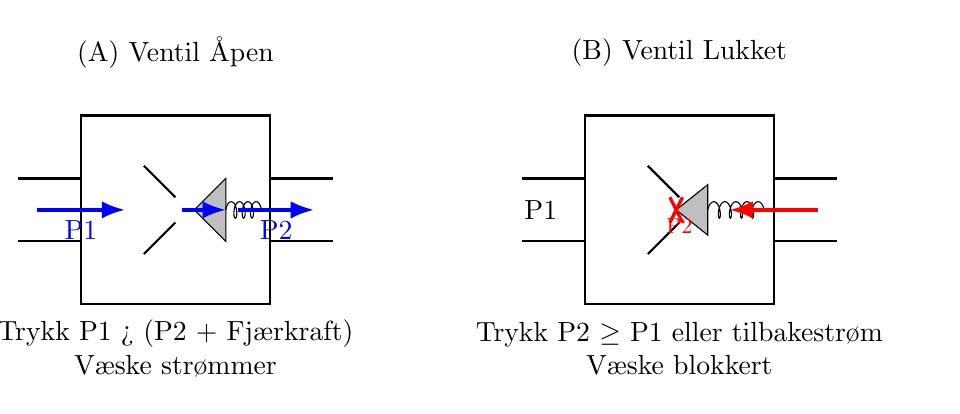
\begin{tikzpicture}[scale=0.8, >=Latex] % Juster scale etter behov

    % --- Del A: Ventil Åpen ---
    \begin{scope}[xshift=-4cm] % Plasserer del A til venstre
        \node at (0, 2.5) {(A) Ventil Åpen};

        % Ventilhus
        \draw[thick] (-1.5, -1.5) rectangle (1.5, 1.5);
        \draw[thick] (-2.5, 0.5) -- (-1.5, 0.5);
        \draw[thick] (-2.5, -0.5) -- (-1.5, -0.5);
        \draw[thick] (1.5, 0.5) -- (2.5, 0.5);
        \draw[thick] (1.5, -0.5) -- (2.5, -0.5);

      % Sete (Venstre side)
      \draw[thick] (-0.5, 0.7) -- (0, 0.2);
      \draw[thick] (-0.5, -0.7) -- (0, -0.2);
      \coordinate (SeatTop) at (-0.5, 0.7);
      \coordinate (SeatBottom) at (-0.5, -0.7);

      % Kjegle/Poppet (Løftet fra setet)
      \coordinate (PoppetTip) at (0.3, 0);
      \coordinate (PoppetTop) at (0.8, 0.5);
      \coordinate (PoppetBottom) at (0.8, -0.5);
      \draw[fill=lightgray] (PoppetTip) -- (PoppetTop) -- (PoppetBottom) -- cycle;

      % Fjær (Komprimert)
      \draw[decoration={coil,aspect=0.4,segment length=3pt,amplitude=3pt},decorate] (0.8, 0) -- (1.4, 0);

        % Strømningspil
        \draw[->, very thick, blue] (-2.2, 0) -- (-0.8, 0) node[below, pos=0.5] {P1};
        \draw[->, very thick, blue] (0.1, 0) -- (0.8, 0); % Gjennom gapet
        \draw[->, very thick, blue] (1.0, 0) -- (2.2, 0) node[below, pos=0.5] {P2};

        % Label P1 > P2 + Fjærkraft
        \node[align=center] at (0, -2.2) {Trykk P1 > (P2 + Fjærkraft) \\ Væske strømmer};

        % Komponent-labels (kan legges til ved behov)
        %\node[pin=120:{Sete}] at (SeatTop) {};
        %\node[pin=60:{Kjegle}] at (PoppetTop) {};
    \end{scope}

    % --- Del B: Ventil Lukket ---
     \begin{scope}[xshift=4cm] % Plasserer del B til høyre
        \node at (0, 2.5) {(B) Ventil Lukket};

        % Ventilhus
        \draw[thick] (-1.5, -1.5) rectangle (1.5, 1.5);
        \draw[thick] (-2.5, 0.5) -- (-1.5, 0.5);
        \draw[thick] (-2.5, -0.5) -- (-1.5, -0.5);
        \draw[thick] (1.5, 0.5) -- (2.5, 0.5);
        \draw[thick] (1.5, -0.5) -- (2.5, -0.5);

        % Sete (Venstre side)
        \draw[thick] (-0.5, 0.7) -- (0, 0.2);
        \draw[thick] (-0.5, -0.7) -- (0, -0.2);

        % Kjegle/Poppet (Mot setet)
        \coordinate (PoppetTipClosed) at (-0.05, 0); % Litt foran setet
        \coordinate (PoppetTopClosed) at (0.45, 0.4);
        \coordinate (PoppetBottomClosed) at (0.45, -0.4);
        \draw[fill=lightgray] (PoppetTipClosed) -- (PoppetTopClosed) -- (PoppetBottomClosed) -- cycle;

        % Fjær (Avslappet/Lett spent)
        \draw[decoration={coil,aspect=0.4,segment length=4pt,amplitude=3pt},decorate] (0.45, 0) -- (1.4, 0);

        % Blokkert strøm (pil fra høyre)
        \draw[->, very thick, red] (2.2, 0) node[below, pos=0.1] {P2} -- (0.8, 0);
        % Stopp-symbol ved setet
        \draw[very thick, red] (PoppetTipClosed) ++(-0.1, 0.2) -- ++(0.2, -0.4);
        \draw[very thick, red] (PoppetTipClosed) ++(-0.1, -0.2) -- ++(0.2, 0.4);
        \node at (-2.2, 0) {P1};

        % Label P2 >= P1 eller Tilbakestrøm
        \node[align=center] at (0, -2.2) {Trykk P2 $\ge$ P1 eller tilbakestrøm \\ Væske blokkert};

     \end{scope}

    \end{tikzpicture}
    \caption{Prinsippskisse av en fjærbelastet tilbakeslagsventil med kjegle (poppet). (A) Viser ventilen åpen for strøm fra venstre mot høyre. (B) Viser ventilen lukket, blokkerer strøm fra høyre mot venstre.}
    \label{fig:tilbakeslagsventil_prinsipp}
\end{figure}

%--- Figur med Hydraulisk Symbol ---
\begin{figure}[ht]
    \centering
    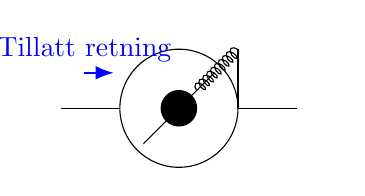
\begin{tikzpicture}[>=Latex, scale=1.5] % Juster scale etter behov

        % Symbol-komponenter
        \draw (0,0) circle (0.5cm); % Ytre sirkel
        \draw[fill=black] (0,0) circle (0.15cm); % Ball
        \draw (-0.3, -0.3) -- (0.3, 0.3); % Sete-linje

        % Fjær
        \draw[decoration={coil,aspect=0.5,segment length=2pt,amplitude=2pt},decorate] (0.15, 0.15) -- (0.5, 0.5);

        % Tilkoblingslinjer
        \draw (-1, 0) -- (-0.5, 0); % Innløp
        \draw (0.5, 0) -- (1, 0);  % Utløp (etter fjær-tilkobling på sirkel, egentlig)
        \draw (0.5,0.5) -- (0.5,0); % Forbinder fjær til utløpslinje
        \draw (0.5,0) -- (0.7,0);  % Korrigert utløpslinje start

        % Strømningsretning (implisitt, men kan legge til pil for klarhet)
        \draw[->, thick, blue] (-0.8, 0.3) -- (-0.55, 0.3);
        \node[blue] at (-0.8, 0.5) {Tillatt retning};

    \end{tikzpicture}
    \caption{Standard hydraulisk symbol for en fjærbelastet tilbakeslagsventil.}
    \label{fig:tilbakeslagsventil_symbol}
\end{figure}

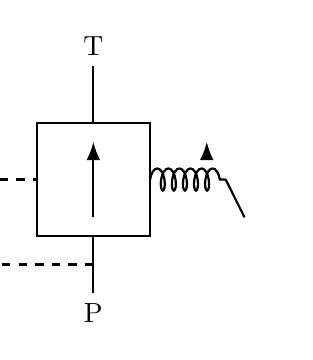
\begin{tikzpicture}[>=Latex, scale=1.2, thick] % Juster scale etter behov

    % Hovedsymbol (firkant)
    \def\ValveSize{1.2} % Størrelse på firkanten
    \draw (0,0) rectangle (\ValveSize, \ValveSize);

    % Porter (P = Trykk inn, T = Tank/retur)
    \coordinate (P_in) at (\ValveSize/2, 0);
    \coordinate (T_out) at (\ValveSize/2, \ValveSize);
    \draw (P_in) -- ++(0, -0.6) node[below] {P}; % Innløp fra trykksiden
    \draw (T_out) -- ++(0, 0.6) node[above] {T}; % Utløp til tank

    % Intern pil (viser potensiell strømningsvei når åpen)
    % Offset for å vise normalt stengt
    \draw [-{Latex}] (\ValveSize/2, 0.2) -- (\ValveSize/2, \ValveSize-0.2);

    % Pilotlinje (føler trykket på P-siden)
    \coordinate (PilotTakeOff) at (\ValveSize/2, -0.3); % Punkt på P-linjen
    \draw[dashed] (PilotTakeOff) -| (-0.5, \ValveSize/2) -- (0, \ValveSize/2); % Styretrykk inn på venstre side

    % Fjær (holder ventilen stengt)
    \coordinate (SpringStart) at (\ValveSize, \ValveSize/2);
    \coordinate (SpringEnd) at (\ValveSize+0.8, \ValveSize/2);
    \draw[decoration={coil, aspect=0.4, segment length=4pt, amplitude=4pt}, decorate]   (SpringStart) -- (SpringEnd);

    % Justeringspil (indikerer at fjærspenningen/åpningstrykket kan justeres)
    \draw [-{Latex}] (\ValveSize+1.0, \ValveSize/2 - 0.4) -- (SpringEnd)+(-0.2, 0.4);
    % Alternativ justeringspil (gjennom fjæren):
    % \draw [-{Latex}] (\ValveSize+0.8+0.2, \ValveSize/2 - 0.4) -- (\ValveSize+0.8-0.2, \ValveSize/2 + 0.4);

    % Forklarende tekst (valgfritt, kan fjernes)
    %\node[align=center, below=1cm of P_in] {Symbol for justerbar \\ trykkbegrensningsventil};

\end{tikzpicture}
\vskip 2.5pt 
\oppgave{}%8
\vskip 2.5pt 
En jekk er utstyrt med en pumpe der stempelet (S1) har et areal på 1 cm². Kraften vi bruker på pumpa, er 600 N. Arealet til stempelet på løftesylinderen (S2) er 20 cm²:
\begin{itemize}
	\item Hvor stor kraft får vi på løftesylinderen?
	\item Hvor mange kilo kan den løfte? 
\end{itemize}
\vskip 5pt 
\vskip 2.5pt 
\newpage
\oppgave{}%9
\vskip 1cm 
Beskrivelse av problemet En dobbeltvirkende sylinder brukes til å åpne og lukke en skottluke. Lukking skal skje uten rykk og skal foregå i en jevn, justerbar hastighet. Hastigheten justeres med en enveis strømningskontrollventil.
\vskip 1cm 
For å sikre at den tunge døren ikke trekker stempelstangen ut av sylinderen under lukkingen, må en trykkavlastningsventil brukes som en motstøtte.
\vskip 1cm 
$$\includegraphics[width=1\textwidth]{../output/noGPLimages/a2INTHydraulikk02.png}$$
\vskip 1cm 
Du skal simulere kretsen i fluidsim. \\
Du skal levere følgende to filer:
\begin{itemize}
	\item dittNavn.cir %(Fil fra fluidsim) 
	\item dittNavn.png %(screenshot fra simulering)
\end{itemize}

Sendes på mail til: fred-olav.mosdal@skole.rogfk.no
med emne: 2INTA
\vskip 1cm 
$$\includegraphics[height=1\textheight]{../output/noGPLimages/a2INTHydraulikk01.png}$$
\vskip 5pt 
\vskip 2.5pt 




\end{document}
